\begin{annexesenv}

% Imprime uma página indicando o início dos anexos
\partannexes

\chapter{INA 326 complete Schematic.}

\begin{figure}[!htpb]
  \centering
  \caption{INA 326 Complete Schematic}
  \label{INA-complete-schematic}
  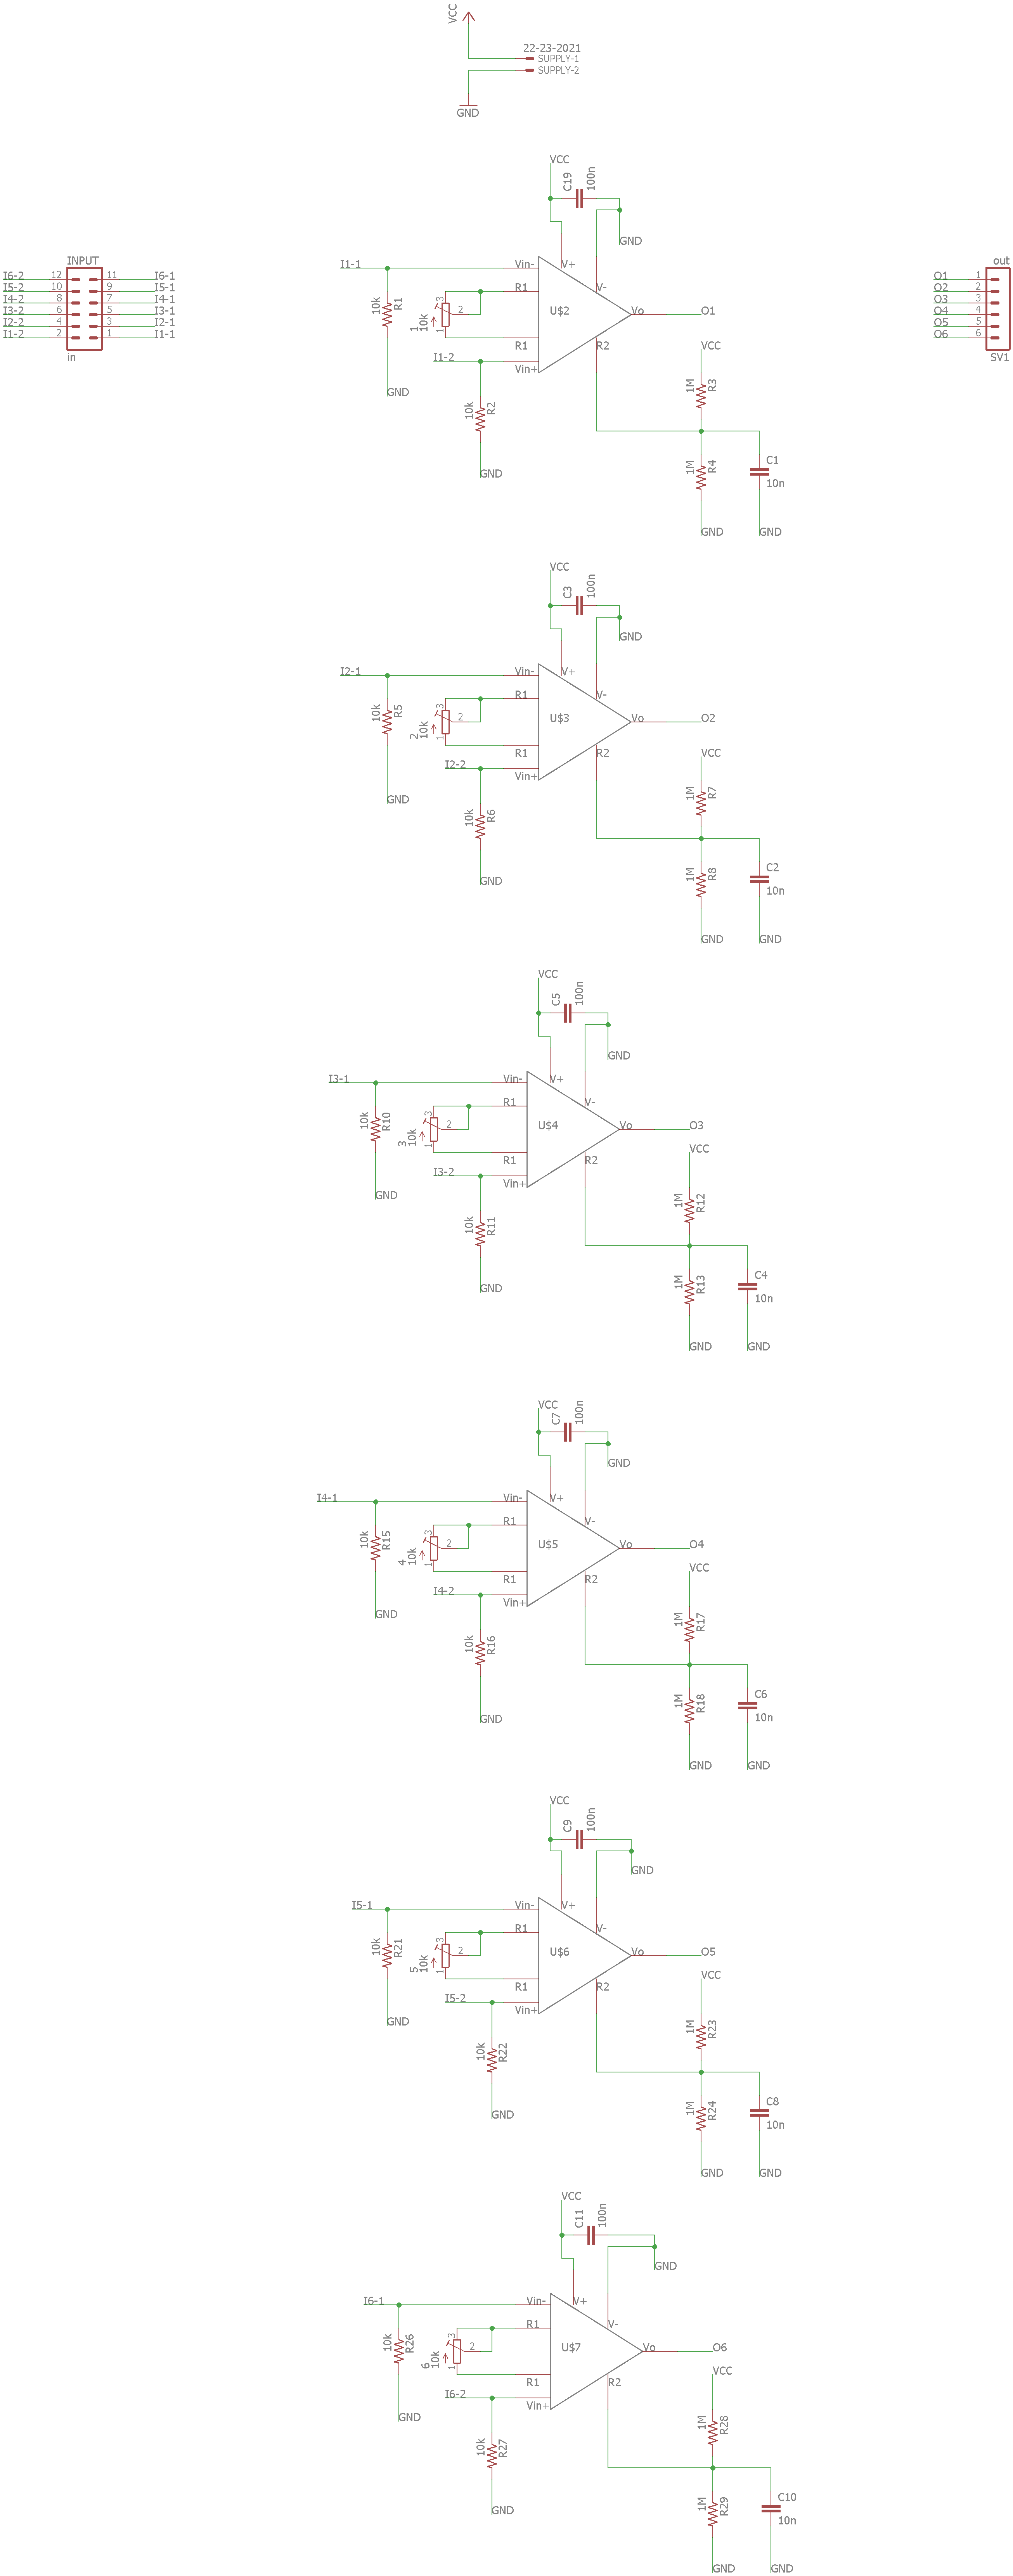
\includegraphics[scale=0.35]{images/INA/complete-schematic}
  \legend{Source: authors}
\end{figure}

\end{annexesenv}

\chapter{Cost Table.}

\begin{table}[htb]
  \begin{center}
    \ABNTEXreducedfont
    \caption[INA Board Cost Table]{INA Board Cost Table}
    \label{Cost-table}
    \begin{tabular}{|c|c|c|}
      \hline
    Componente & Quantidade & Custo \\ \hline
    INA326 & 6 & TODO\\ \hline
    10k$\Omega$ Trimmer Potentiometer & 6 & 7,50 \\ \hline
    10nF Ceramic Capacitor & 6 & 1,00 \\ \hline
    100nF Electrolytic Capacitor & 6 & 1,50 \\ \hline
    10k$\Omega$ Resistor & 12 & 2,00 \\ \hline
    1M$\Omega$ Resistor & 12 & 2,00 \\ \hline
    Pin bar 1x40 & 1 & 3,00 \\ \hline
    Pin bar 2x40 & 1 & 7,00 \\ \hline
  \end{tabular}
  \legend{Source: authors}
\end{center}
\end{table}
